% Made up for the tikra benchmark.
\usetikzlibrary{arrows.meta}
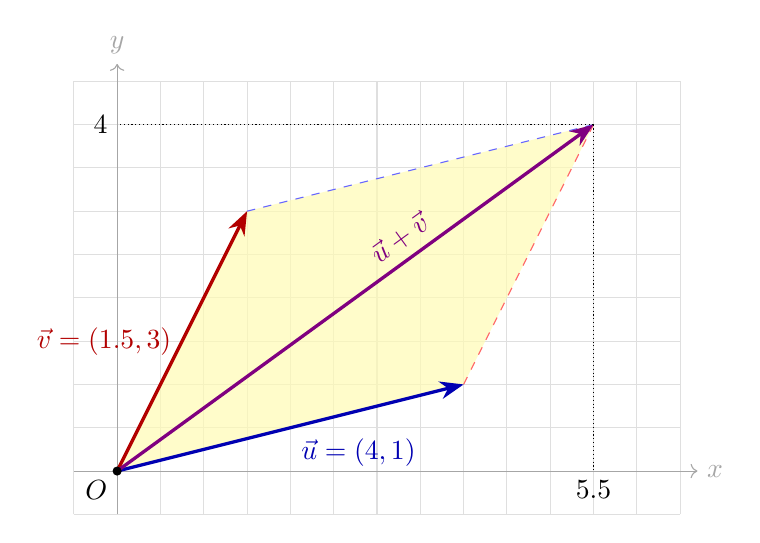
\begin{tikzpicture}[scale=1.1, vec/.style={-{Stealth[length=3mm]}, very thick}]
  \draw[gray!25, step=0.5] (-0.5,-0.5) grid (6.5,4.5);
  \draw[gray!70, ->] (-0.5,0) -- (6.7,0) node[right] {$x$};
  \draw[gray!70, ->] (0,-0.5) -- (0,4.7) node[above] {$y$};
  \coordinate (O) at (0,0); \coordinate (U) at (4,1); \coordinate (V) at (1.5,3);
  \coordinate (S) at (5.5,4);
  \fill[yellow!30, opacity=0.7] (O) -- (U) -- (S) -- (V) -- cycle;
  \draw[dashed, blue!60] (V) -- (S);
  \draw[dashed, red!60] (U) -- (S);
  \draw[vec, blue!70!black] (O) -- node[below right] {$\vec u = (4,1)$} (U);
  \draw[vec, red!70!black] (O) -- node[left] {$\vec v = (1.5,3)$} (V);
  \draw[vec, violet] (O) -- node[sloped, above, pos=0.62] {$\vec u + \vec v$} (S);
  \draw[densely dotted] (S) -- (S |- O) node[below] {$5.5$};
  \draw[densely dotted] (S) -- (S -| O) node[left] {$4$};
  \fill (O) circle (1.5pt) node[below left] {$O$};
\end{tikzpicture}
